\clearpage
\newpage
\onecolumn
\appendices
\section{Figures and Tables}

\begin{figure}[H]
    \centering
    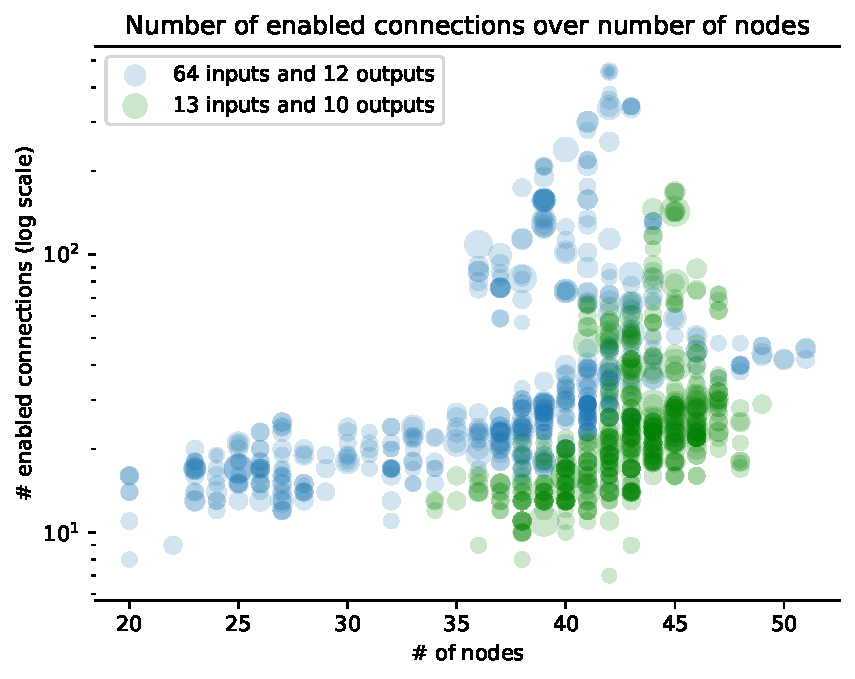
\includegraphics[width=0.6\linewidth]{./images/n_enabled_connections_over_n_nodes_derk_neat.pdf}
    \caption{Number of enabled connections (in logarithmic scale) over number of nodes of a NEAT solver on Derk environment for the best network at each generation. The size of scatters represents the fitness value of the agent. No emerging pattern can be noticed between the decrease of enabled connections over time and the number of nodes.}
    \label{fig:enabled-connection-nodes-derk-neat}
\end{figure}

\begin{figure}[H]
    \centering
    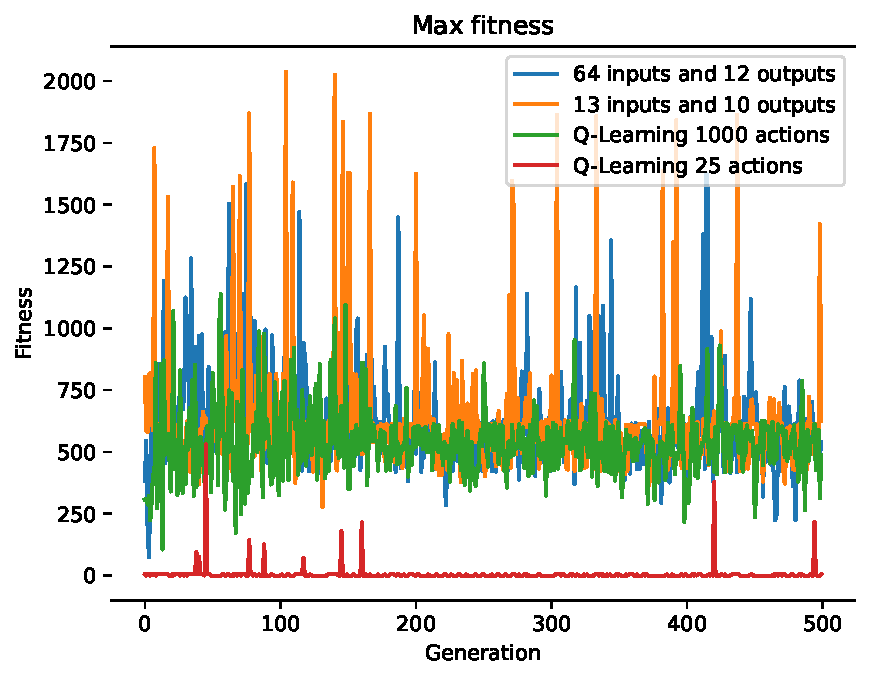
\includegraphics[width=0.6\linewidth]{./images/fitness_over_iterations_derk_neat.pdf}
    \caption{Best fitness over generations on different NEAT attempts on the Derk environment, low performances of the Q-learning 25 actions are a consequence of the different range of the abilities and the low probability of moving enough close to enemies.}
    \label{fig:fitness-neat-derk}
\end{figure}



% \begin{table*}
%     \caption{BT node output}
%     \begin{center}
%         \begin{tabular}{lccc}
%             \toprule
%             Node type & Succeeds & Fails & Running \\
%             \midrule
%             Fallback & If one child succeeds & If all children fail & If one child returns Running \\
%             Sequence & If all children succeed & If one child fails & If one child returns Running \\
%             Action & Upon completion & Impossible to complete & During completion \\
%             Condition & If true & If false & Never \\
%             \bottomrule
%         \end{tabular}
%     \end{center}
%     \label{tab:bt-node-output}
% \end{table*}

\begin{table*}
    \caption{Performance summary}
    \begin{center}
        \begin{tabular}{llrrrr}
        \toprule
        {}   &  Env & Generation &  Max fitness &        Mean &         Std \\
        Name &  &  &  &  &  \\
        \midrule
        BT          & Frozen Lake & 72 & 0.94 &  -0.0482 & 0.1347 \\
        NEAT        & Frozen Lake & 1 & 1 &  0.00500 & 0.07053 \\
        BT          & Lunar Lander & 654 &  291 &  -132.377  & 187.8  \\
        NEAT        & Lunar Lander & 500 &  281.036445 &  -85.143571 & 238.081605 \\
        BT          & Derk &  500 &  1086.568 & -172.413   & 298.638  \\
        64 inputs and 12 outputs & Derk & 414 & 1627.199951 &  -41.238786 & 461.072898 \\
        13 inputs and 10 outputs & Derk & 104 & 2038.612549 & -108.815655 & 713.525290 \\
        Q-Learning 1000 actions  & Derk &  56 & 1138.235474 & -122.275397 & 378.131604 \\
        Q-Learning 25 actions    & Derk &  45 &  530.440002 &    7.012384 & 101.492292 \\
        \bottomrule
        \end{tabular}
    \end{center}
    \label{tab:performance-summary}
\end{table*}


% \pagebreak
\begin{figure}
    \centering
    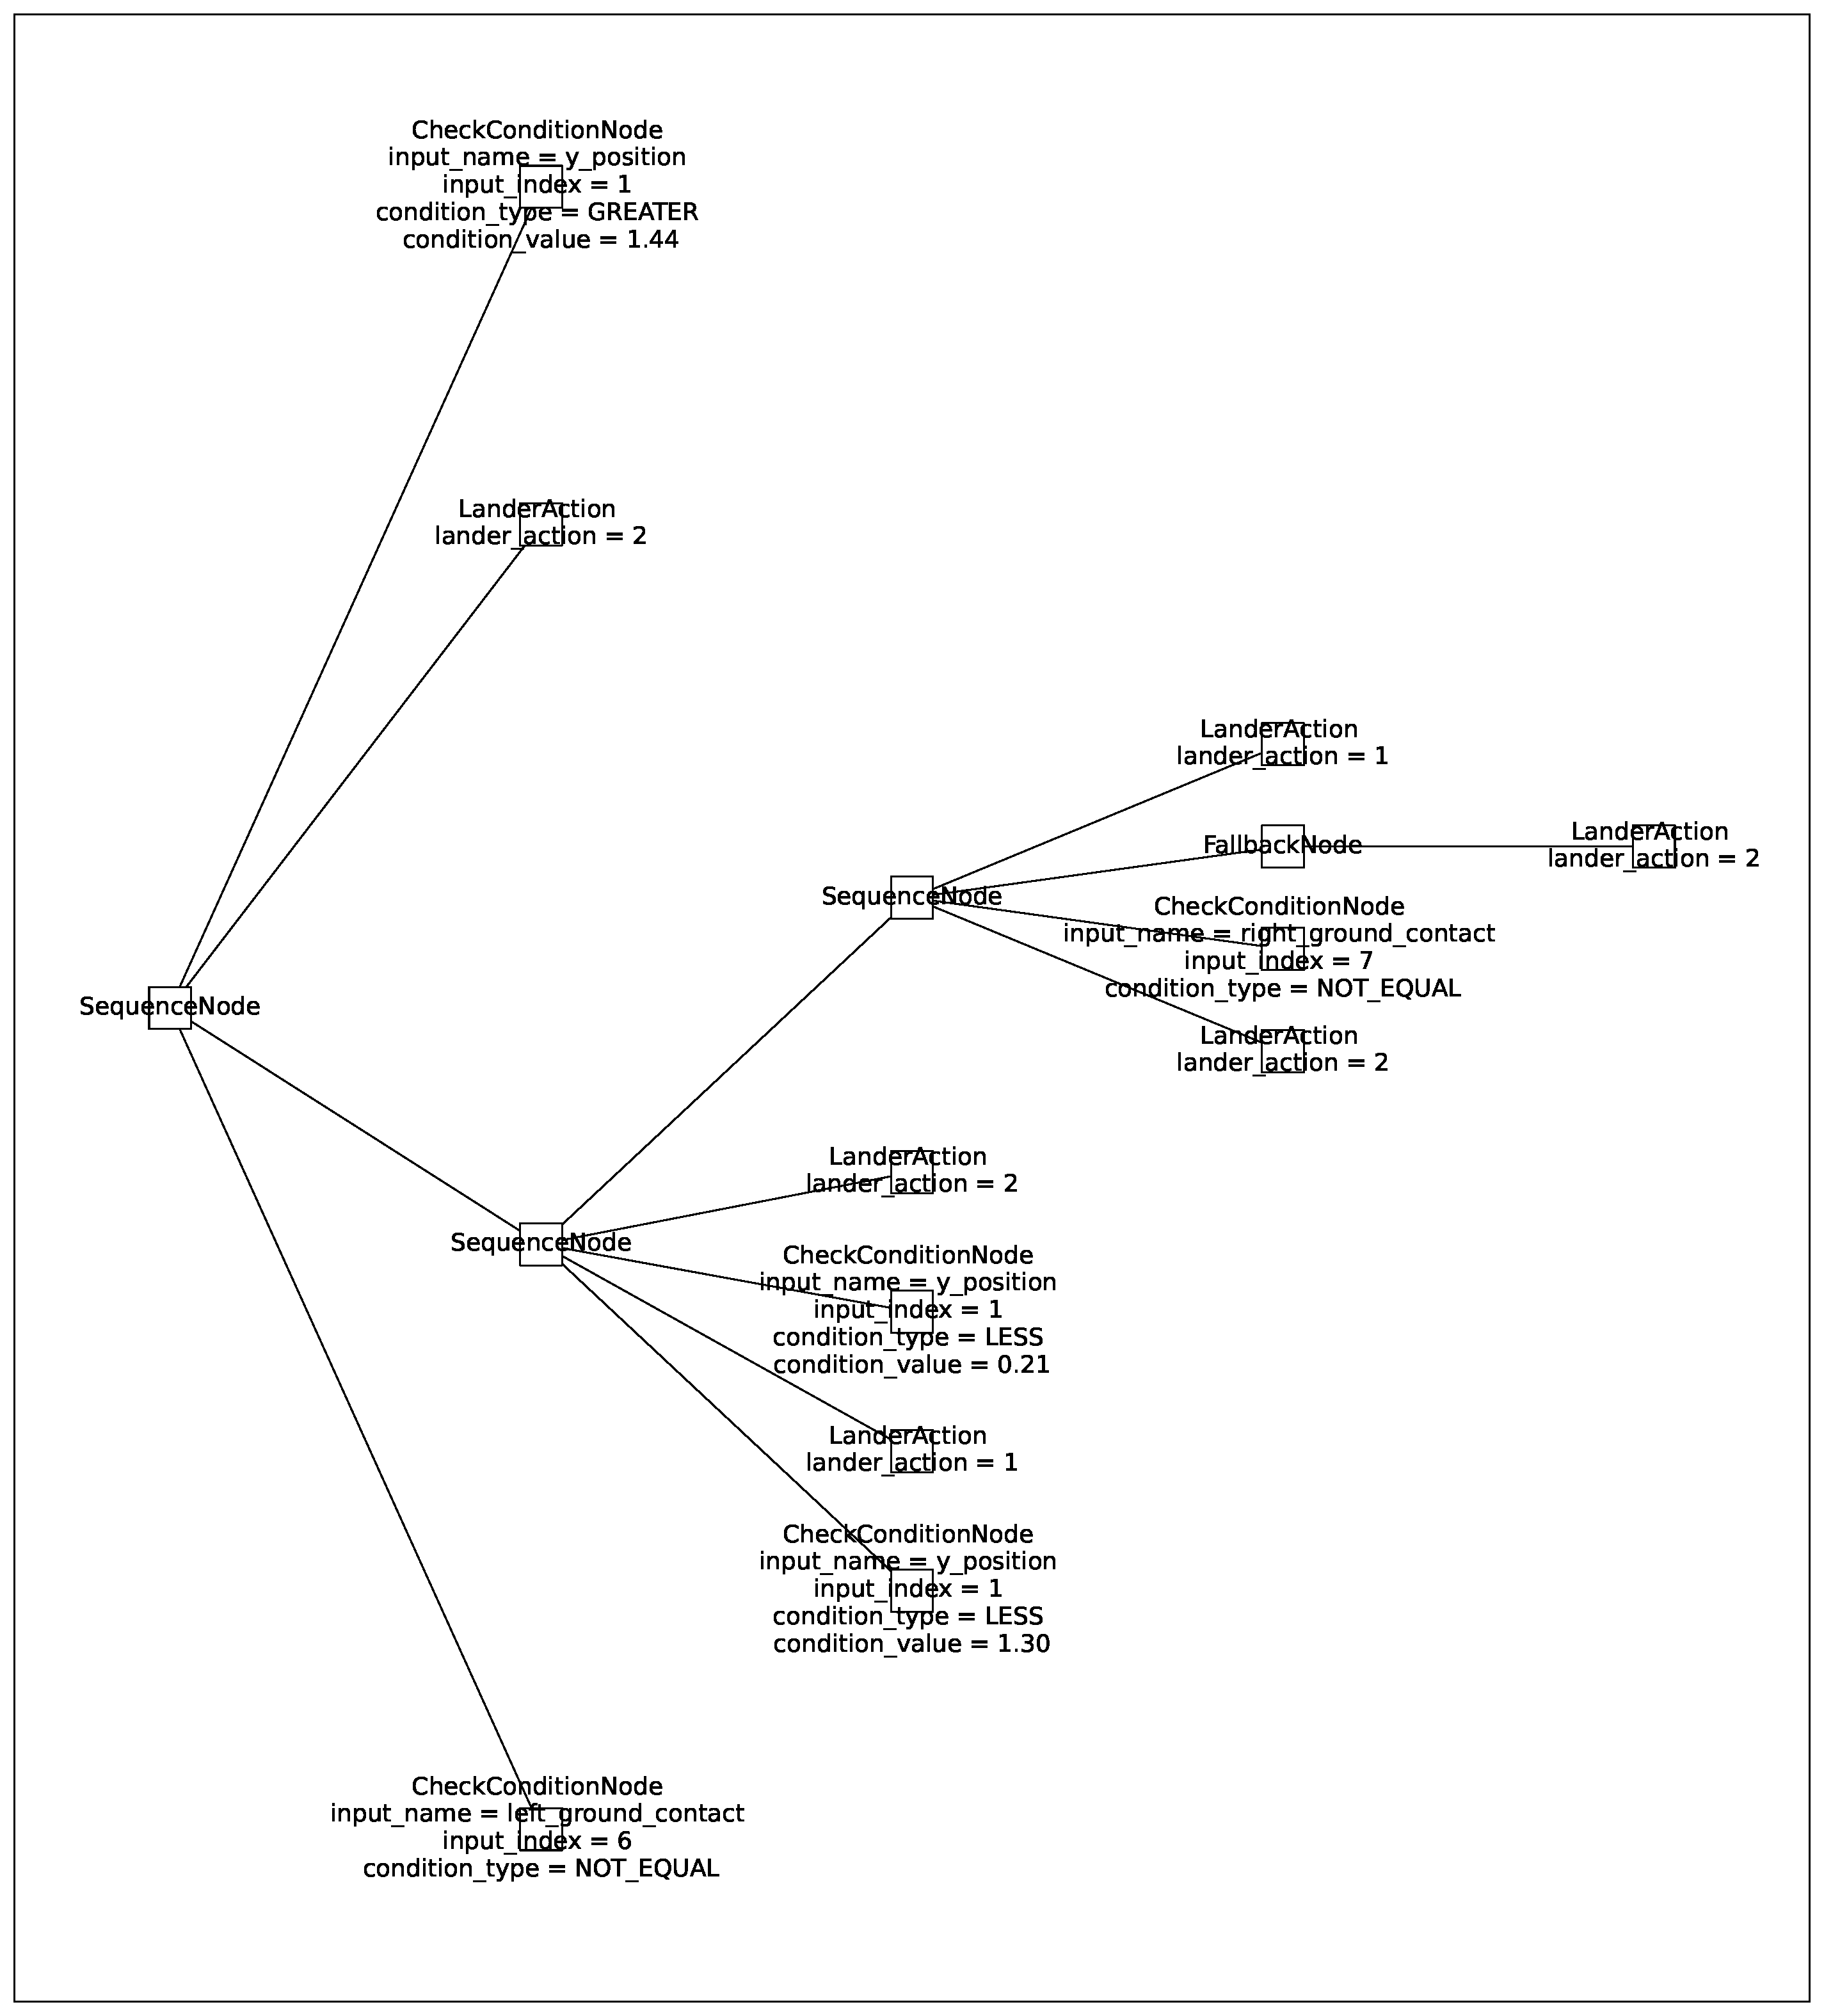
\includegraphics[width=1\linewidth]{./images/lander_BT.pdf}
    \caption{Visual representation of the best BT for Lunar Lander with the root as the leftmost node. The tree nodes are traversed from left to right and from bottom to top in a DFS-like fashion. We can see from the condition nodes that the Lander completely ignores every other input except its y position, which is probably one key element that prevents generalization of this tree on other random seeds. }
    \label{fig:lander-bt-figure}
\end{figure}
